\documentclass[11pt,a4paper]{article}
\usepackage{bbm,amsthm,amsfonts,amssymb,amsmath,latexsym,epic,eepic}
\usepackage{marvosym,graphicx,fancyhdr,bbm, hyperref}
%% \usepackage[dvips]{color}
\usepackage[rflt]{floatflt}
\usepackage{colortbl}
\usepackage[ngerman]{babel}

\definecolor{Grey}{rgb}{0.5,0.5,0.5}
\definecolor{Red}{rgb}{1.0,0.0,0.0}

\usepackage{typearea}
\areaset{156mm}{235mm}
%\setlength{\parskip}{5pt plus 2pt minus 1pt}
\setlength{\parindent}{0pt}

% use \M for matrices and \V for vectors in math mode
\newcommand{\M}[1]{\mathbf{#1}}
\newcommand{\V}[1]{\mathbf{#1}}
\newcommand{\norm}[1]{\left | \left | #1 \right | \right |}
\newcommand{\RR}{\mathbbm{R}}        % set of real numbers


\renewcommand\floatpagefraction{0.8}
\renewcommand\topfraction{1}
\renewcommand\bottomfraction{0.9}
\renewcommand\textfraction{0.0}
%\def\dbltopfraction{1.0}
%\def\bottomfraction{1.0}
%\def\dblfloatpagefraction{0.8}


\makeatletter
\renewenvironment{thebibliography}[1]
     {\section*{\refname}%
      \@mkboth{\MakeUppercase\refname}{\MakeUppercase\refname}%
	 \parsep0mm
	 \itemsep0mm
	 %\labelsep0mm
	 %\itemindent0mm
      \list{\@biblabel{\@arabic\c@enumiv}}%
           {\settowidth\labelwidth{\@biblabel{#1}}%
            \leftmargin\labelwidth
            \advance\leftmargin\labelsep
            \@openbib@code
            \usecounter{enumiv}%
            \let\p@enumiv\@empty
            \renewcommand\theenumiv{\@arabic\c@enumiv}}%
      \sloppy
      \clubpenalty4000
      \@clubpenalty \clubpenalty
      \widowpenalty4000%
      \sfcode`\.\@m}
     {\def\@noitemerr
       {\@latex@warning{Empty `thebibliography' environment}}%
      \endlist}
\renewcommand\newblock{\hskip .11em\@plus.33em\@minus.07em}
\let\@openbib@code\@empty
\makeatother

\begin{document}

\title{\Large \bf Abgabe zum Praktikum Mess- und Regelungstechnik \\ \textbf{Revision 1}}

\author{Simon Klüpfel, Lukas Zeller\\
  Robotik und Telematik \\
  Universität Würzburg\\
  Am Hubland, D-97074 Würzburg\\
{\small \texttt{simon.kluepfel@stud-mail.uni-wuerzburg.de, lukas.zeller@stud-mail.uni-wuerzburg.de}}
}
\date{17. November 2022}

\maketitle

\section{Einleitung}
1020 PS auf 2162kg, und von 0 auf 100 km/h in 2,1 Sekunden\cite{website:tesla}. Dazu noch ein Level an autonomen Fahren das uns wie von Zauberhand durch den Verkehr bringt
und die kognitiven Faehigkeiten des Menschen teilweise bereits uebersteigt. Die Rede ist vom Tesla Model S. Die enormen Fahrleistungen lassen sich durch modernsten Maschinenbau und Elektrotechnik 
sowie jahrelanger Entwicklung erreichen. Spannender ist nach Meinung der Autoren schon das (teil-)autonome Fahren und die Fortbewegung eines 
zwei Tonnen schweren Fahrzeugs in einer dynamischen Umgebung wie dem Strassenverkehr, ohne einen Unfall zu verursachen oder im Worst-Case Menschen zu verletzen oder gar zu toeten.
Dass dies nicht passiert spricht einmal fuer das Know-How der Tesla-Ingenieure als auch der Zuverlaessigkeit der verwendeten Technik. In dieser Arbeit wird 
ein kleiner Einblick in die Technologie der Lokalisierung gegebenen und ein Vergleich angestellt zwischen zwei Methoden, der AMCL- und Odometrie-Lokalisierung.

\section{Zur Lokalisierung}
Aus \cite{website:lokalisierung}, Folie 5-2, lassen sich drei Grundvoraussetzungen sowie das Ziel fuer unsere Roboterlokalisierung definieren: Er bewegt sich in der Umgebung mittels bekannter Stuerbefehle,
nimmt seine Umwelt mit Sensoren wahr und hat eine Karte seiner Umgebung zum Abgleich gespeichert. Das Ziel ist eine Positonsabschaetzung zum Zeitpunkt t in X- und Y-Position sowie ein Heading welches
die Richtung angibt. Als Referenz ist ein in der Umgebung verankertes Koordinatensystem gegeben. Weiter unterscheidet man zum Beginn der Lokalisierung zwischen lokaler und globaler
Selbstlokalisierung. Im ersten Fall ist die Initialposition des Roboters grob bekannt, das Ziel ist es bei Bewegung des Roboters eine Neuberechnung der Position durchzufuehren,
dieses Verfahren nennt man \textit{position tracking}. Bei der schwierigeren globalen Selbstlokalisierung kennen wir unsere Initialposition dagegen nicht, sie muss aus der 
Roboterbewegung und neugewonnenen Sensordaten errechnet werden. Hier kann das \textit{kidnapped robot problem} eine Rolle spielen, bei der der Roboter in Zuge einer nicht abgeschlossenen Lokalisierung
umgesetzt wird.
Bei der Sensorik die zur Lageschaetzung verwendet wird unterscheidet man zwischen \textit{propriozeptiven}, d.h. internen, und \textit{exteriozeptiven}, externen, Sensoren. 
Ersteres misst die lokal am Roboter anfallenden \textit{onboard} \cite{website:robotik} Eigenschaften wie die Drehzahl der Radmotoren oder die Temperatur, die 
exteriozeptiven Sensoren liefern Messungen aus der Umgebung des Roboters, als Beispiel nennt \cite{website:robotik} Distanzmessungen wie Ultraschall, Laser, oder eine Kameraaufnahme der Umgebung.
\section{Kurze Einführung in den Volksbot und ROS}
In dieser Arbeit wurde das Robot Operating System, kurz \textit{ROS}, auf einem Roboter, dem \textit{Volksbot} verwendet.
Der verwendete Roboter ist der \textit{RT3-2} mit zwei bzw. einem (\textit{RT-3}) passiven Rad und jeweils zwei angetriebenen Raeder die vorne rechts und links angebracht sind.
Entwickelt wurden diese vom \textit{Fraunhofer Institut IAIS} aus Sankt Augustin. 
Die technischen Daten sind wie folgt:\\
\vspace{-5mm}
\begin{center}
\begin{tabular}{| p{5cm} p{5cm} |}
  \hline
  Abmessungen & 580x520x315mm (L x B x H) \\
  Gewicht & 17kg \\
  
  Raddurchmesser & 260x85mm (aktive Räder) \\
   & 200mm (passive Räder) \\
  Maximale Geschwindigkeit & 2,2 $\frac{m}{s}$ \\
  
  Maximale Zuladung & 25kg \\
  \hline
\end{tabular} \\
\end{center}

\textit{Daten aus} \cite{website:volksbot} \\

Auf dem Roboter ist ein Laserscanner sowie Hardware zur Verbindung mit dem als ROS-Plattform verwendeten
Laptop installiert. Neben der Steuerung beziehungsweise Regelung ueber \textit{ROS} lässt sich der Roboter über einen Joystick, ähnlich eines Gamecontrollers, manuell steuern.
Das \textit{Robot Operating System}  entstand aus dem Bedarf fuer ein Open-Source-Roboter-Framework in der Robotercommunity.
Es entstand Mitte der 2000er-Jahre aus Projekten an der \textit{Stanford University} wie dem \textit{STanford AI Robot - STAIR}.
2007 konnte mithilfe von \textit{Willow Garage Inc}, einer amerikanischen Robotikfirma, und derer
Resourcen die ROS-Konzepte in erste Implementationen umgesetzt werden. Heute hat \textit{ROS} zehntausende Nutzer auf der ganzen Welt,
die Anwendungen reichen von Amateurrobotern bis zu grossen automatisierten Industrieanlagen. 
\textit{ROS} an sich besteht dabei aus vielen kleinen Programmen die ueber Nachrichten, die \textit{Messages}, miteinander kommunizieren.
Die Nachrichten werden dabei untereinander direkt verschickt ohne einen zentralen Bus oder aehnliches. Insgesamt
folgt \textit{ROS} damit einer Graphenarchitektur mit Knoten (englisch \textit{nodes}) und Kanten (\textit{edges}), sie entsprechen den Nachrichten. \cite{quigley2015programming}
Es werden sowohl vorgegebene ROS-Nodes, die vom Institut für Robotik und Telematik zur Verfügung gestellt wurden, als auch angepasste Nodes die die Autoren selbst erstellt beziehungsweise
geändert haben, verwendet. 
\section{Odometrie, GMapping und AMCL im Überblick}
\subsection*{Die Odometrie}
Die Odometrie errechnet die Bewegung des Roboters ueber die Radgeschwindigkeit und \\ -bewegung 
des \textit{Volksbot}. Im Zentrum dieser Rechnung stehen die mathematischen Zusammenhaenge im Kreisbogen. 
Aus \cite{website:dresden} wurde dazu folgende Grafik entnommen:

\begin{figure}[ht]
  \centering
  \includegraphics[width = 12cm]{kreisbogen.png}
  \caption{Ein Kreissegment mit verschiedenen eingezeichneten Boegen bei unterschiedlichen Radien. Die Radienlaengen sind an der oberen Kreiskante 
  aufgetragen. Der Winkel $\alpha$ des Kreissegments ist an der Spitze eingezeichnet}
  \label{fig: Kreissegment}
\end{figure}


\cite{olson2004primer} stellt die Grundzuege dieses Verfahrens vor. Hierzu betrachte man zuerst folgende 
Abbildung und die geometrischen Zusammenhaenge:

\begin{figure}[ht]
  \centering
  \includegraphics[width = 12cm]{odometry.png}
  \caption{Die Geometrie der Odometrie, aus \cite{olson2004primer}. \textit{OLSON} schreibt dazu: \textit{ Detailed odometry geometry. 
  We compute the center of the circle P by forcing $d_{left}$ and $d_{right}$ to be two arcs with the same inner angle $\phi$.
  From this, we can compute the new robot position $(x', y', \theta')$}}
  \label{fig: Odometrie}
\end{figure}



\section{Die Funktionsweise der Pfadverfolgung und ihre Güte}

\section{Experimenteller Vergleich der Qualität der Pfadverfolgung bei Verwendung von AMCL-  bzw. Odometrie-Lokalisierung}
Nun soll betrachtet werden wie genau die Lokalisierungsmethoden einen vorgegebenen Pfad verfolgen. Desweiteren soll ein Vergleich zwischen beiden Methoden angestellt werden. 
Demnach ist die Lokalisierungsmethode besser, welche in der Verwendung eine geringere Abweichung vom vorgegebenen Pfad aufweist. 
Wir gaben dem Controller hier einen Pfad vor, welcher mit Hilfe der 3D-Design-Applikation \textit{Blender} so erstellt wurde, dass er sowohl
gerade Linien als auch weiche und harte Kurven enthält.

\begin{figure}[ht]
\centering
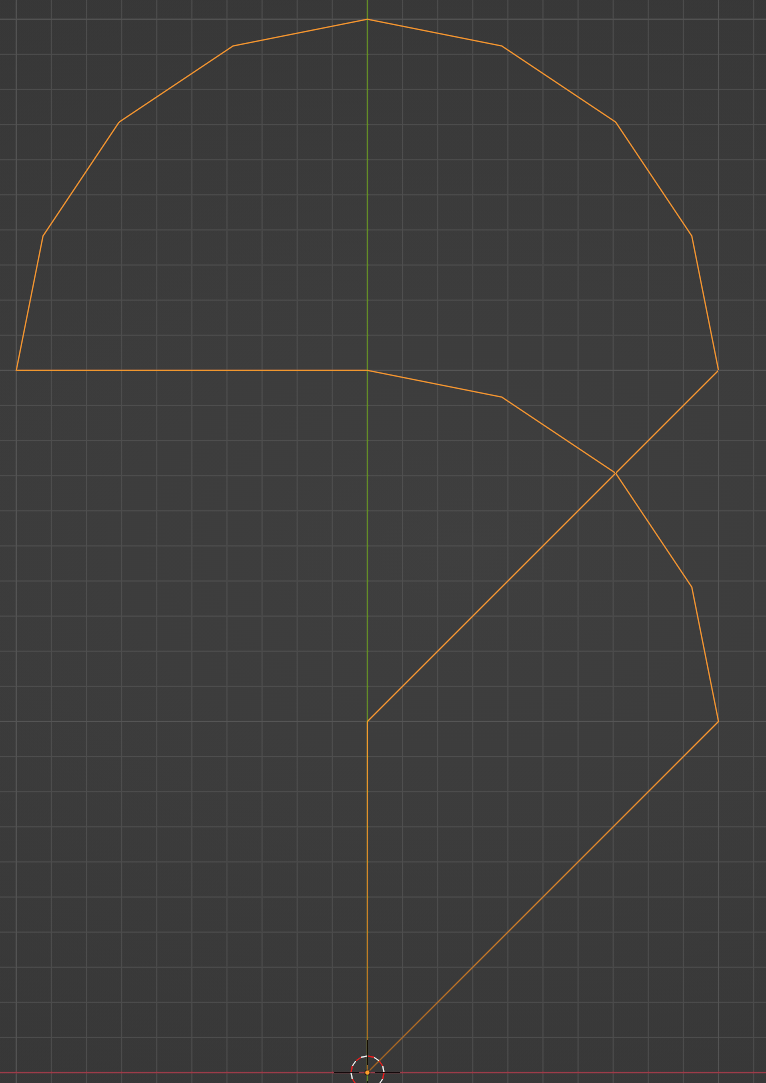
\includegraphics[scale = 0.6]{pfadgrafik.png}
\caption{Der Pfad, wie er in Blender erstellt wurde. Man erkennt eine Linienstruktur bestehend aus gerade und gekurvten Teilstrecken, die einen geschlossenen Pfad bilden}
\label{fig: MessungExperiment}
\end{figure}

Start und Ende sind hier der Cursor unten im Bild, Anfangsrichtung ist gerade nach oben. Die verwendete Pfaddatei ist in \verb+catkin_ws+ als 
\verb+Pfad.dat+ zu finden.
Dieser Pfad wurde auf dem Boden des Testgeländes mit Wollfäden markiert. Der Controller hat die Koordinaten des erstellten Pfades 
als relativ interpretiert. Dadurch konnten wir den Roboter am Startpunkt des Pfades platzieren, und in die Geradeaus-Richtung des Pfades orientieren. 
Dies wurde mithilfe durch ein Maßband, das durch die gerade Mittellinie des Pfades bis zum Roboter führt, und diesen dann symmetrisch teilt, möglichst exakt getan. 
Dazu wurde im Ursprung des Roboters in der Mitte der Vorderradachse ein Schraubenzieher befestigt, der gerade nach unten zeigt um die Position auf dem 
Boden leichter einsehen zu können. Es ergibt sich dennoch ein systematischer Fehler, da die Startausrichtung und -Platzierung des Roboters nicht perfekt 
mit der des Pfades am Boden übereinstimmt. Der geschätzte Maximalfehler für die Position des Roboters beträgt 2cm, der der Ausrichtung 2°. 
\\Dadurch ergibt sich im maximalen Abstand vom Startpunkt ein maximaler Fehler von: \\
$
0,02m + tan(2^\circ) * 3m = 0,12m
$                                                          \\ 
An allen anderen Orten ist der systematische Fehler durch den geringeren Abstand vom Startpunkt kleiner.
Nachdem der Roboter platziert wurde, wurde ein Node gestartet das den benannten Pfad abfährt, und dabei alle 2 Sekunden anhält, sodass seine Position 
auf dem Boden markiert werden kann. Dies wird für beide Lokalisierungsmethoden durchgeführt. Danach wird der senkrechte Abstand jedes Punktes 
zum markierten Pfad gemessen und in einer Tabelle eingetragen. Die Messergebnisse sind in Anhang\footnote{Siehe Tabelle 1} einzusehen.

\section{Beschreibung der Ergebnisse}
Der auf dem Boden markierte Pfad und die markierten Punkte, an denen der Roboter anhielt. Diese wurden jeweils auf einem Bild in Blau bei der Pfadverfolgung 
unter Verwendung von AMCL, und in Rot bei der Verwendung von Odometrie, zusätzlich zur besseren Sicht nachbearbeitet, eingekreist und mit der jeweiligen Nummer 
des Anhaltens gekennzeichnet, startend bei 0 für die Initialposition.
Man beobachtet das der Pfad anfangs, bis etwa Punkt 7, mit beiden Lokalisierungsmethoden etwa gleich gut verfolgt wird. Der Durchschnitt der Abweichungen vom Pfad 
von Haltepunkt 1 bis zu Haltepunkt 7 liegt bei Odometrie bei 8cm, bei AMCL 4,2cm. Die folgenden Punkte zeigen bei beiden Lokalisierungsmethoden eine deutlich 
größere Abweichung auf: Punkte 8-13 bei der Verwendung von Odometrie haben eine durchschnittliche Abweichung von 51,2cm, bei der Verwendung von AMCL ist bei den 
Punkten 8-14 eine durchschnittliche Abweichung von 22,9cm aufgetreten. Hierbei ist zu bemerken dass durch das beiden Ansätze in der Realität stark 
verschiedene Pfade verfolgt wurden (siehe Abbildung) und es dazu kam dass AMCL einen längeren Weg zurückgelegt hat, und somit einen Haltepunkt mehr in der Messtabelle 
aufweist als Odometrie.  Anhand der Markierungen auf dem Boden erkennt man auch dass der Odometrie-Ansatz sich nach Haltepunkt 7 durchgehend auf einer Seite des 
zu verfolgenden Pfades befindet, und immer weiter in diese Richtung von diesem abdriftet, während der AMCL Ansatz die Seite wechselt, in welche der Positionsfehler vorliegt.

\section{Diskussion und Auswertung der Fahrtwege unter AMCL und Odometrie}
Die durchschnittliche Abweichung aller Fehlerpunkte von AMCL liegt bei 12,6cm, bei der Odometrie sind es 25,9cm. Zu Beginn der Verfolgung des Pfades lagen beide Methoden 
etwa gleich nahe am Zielpfad, jedoch fing die Odometrie-Lokalisation  ab der ca. Hälfte des Pfades an eine immer größer werdende Abweichung vom Zielpfad aufzubauen bis 
zu einem maximal gemessenem Fehler von 1,13m, während bei AMCL keine größere Pfadabweichung als 36cm gemessen wurde. Das bereits beschriebene Abdriften der 
Haltepunkte des Odometrie Ansatz lässt darauf schließen das die sich akkumulierenden Fehler in den Radumdrehungen, welche das alleinige Lokalisierungsmerkmal 
der Odometrie ist, einen Drift in der Positionierung verursachen, was bewirkt das Odometrie für eine Lokalisierung auf Pfaden, die nicht kurz sind, keine der Realität 
akkuraten Ergebnisse liefern kann. Da AMCL nicht allein auf die Radumdrehungen angewiesen ist, kann es die Fehler dieser Informationsquelle ausgleichen und so auch auf 
längeren Pfaden bis zu einem gewissen Grad die Position genau bestimmen.

\section{Zusammenfassung und Ausblick}

{%\small                   % use small if you need it
\bibliographystyle{plain}
\bibliography{paper}       % use a bib-file paper.bib to collect your references
}

\end{document}

